%%%%%%%%%%%%%%%%%%%%%%%%%%%%%%%%%%%%%%%%%
%
% (c) 2022 by Jennifer Laaser
%
% This work is licensed under the Creative Commons Attribution-NonCommercial-ShareAlike 4.0 International License. To view a copy of this license, visit http://creativecommons.org/licenses/by-nc-sa/4.0/ or send a letter to Creative Commons, PO Box 1866, Mountain View, CA 94042, USA.
%
% The current source for these materials is accessible on Github: https://github.com/jlaaser/pogil-polymers
%
%%%%%%%%%%%%%%%%%%%%%%%%%%%%%%%%%%%%%%%%%

\renewcommand{\figpath}{content/polymphys/thermal-transitions/crystals/figs}
\renewcommand{\labelbase}{crystals}

\begin{activity}{Polymer Crystals}

\begin{instructornotes}
	This activity introduces students to concepts related to crystallization of polymeric materials.
	
	After completing this activity, students will be able to:
	\begin{enumerate}
		\item \dots
	\end{enumerate}
	
	\subsection*{Activity summary:}
	\begin{itemize}
		\item \textbf{Activity type:} Learning Cycle
		\item \textbf{Content goals:} See above %Glass Transitions of Polymer Materials
		\item \textbf{Process goals:} %https://pogil.org/uploads/attachments/cj54b5yts006cklx4hh758htf-process-skills-official-pogil-list-2015-original.pdf
			\begin{enumerate}
				\item Interpreting schematics and equations
				\item Linking concepts to derive a key result
				\item Written and oral communication of reasoning
			\end{enumerate}
		\item \textbf{Duration:} TBD
		\item \textbf{Instructor preparation required:} none beyond knowledge of relevant content
		\item \textbf{Related textbook chapters:}
			\begin{itemize}
				\item \emph{Polymer Chemistry} (Hiemenz \& Lodge), 2nd ed.: TBD
				\item \emph{Introduction to Polymers} (Young \& Lovell), 3rd ed.: TBD
			\end{itemize}
		%\item \textbf{Instructor notes:}
		%	\begin{itemize}
		%		\item \dots
		%	\end{itemize}
	\end{itemize}
	
\end{instructornotes}


\begin{model}[Structures of Polymer Crystals]
	\label{\labelbase:mdl:crystalstructs}
	
	Under the right conditions, some polymers can arrange into highly-ordered, crystalline materials. One common crystalline polymer is poly(ethylene).  A representative structure of crystalline poly(ethylene) is shown below:
	
	\vspace{6pt}
	\centerline{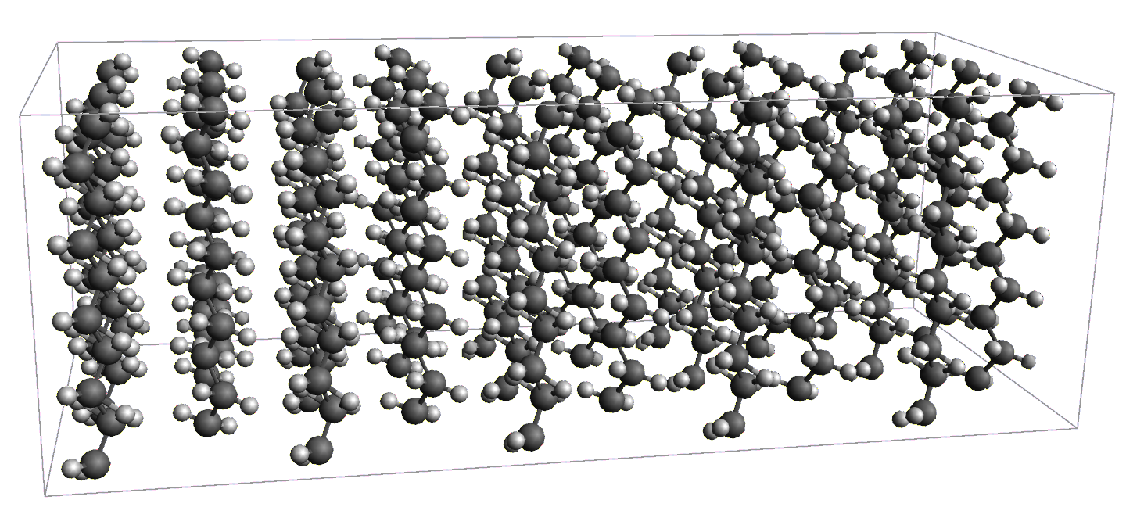
\includegraphics[width=0.6\textwidth]{\figpath/Model1_PE_supercell.pdf}}	
	
	% note for rendering: crystallographic parameters for poly(ethylene) are taken from DOI 10.1039/TF9393500482
	% unit cell dimensions are (7.40, 4.93, 2.534) Angstroms
	% fractional positions of carbon atoms are (0.038, 0.935, 0.250); (0.962, 0.065, 0.750); (0.462, 0.453, 0.750); (0.538, 0.565, 0.250)
	
	A single layer of this crystal, as viewed from the front, appears as follows:
	
	\vspace{6pt}
	\centerline{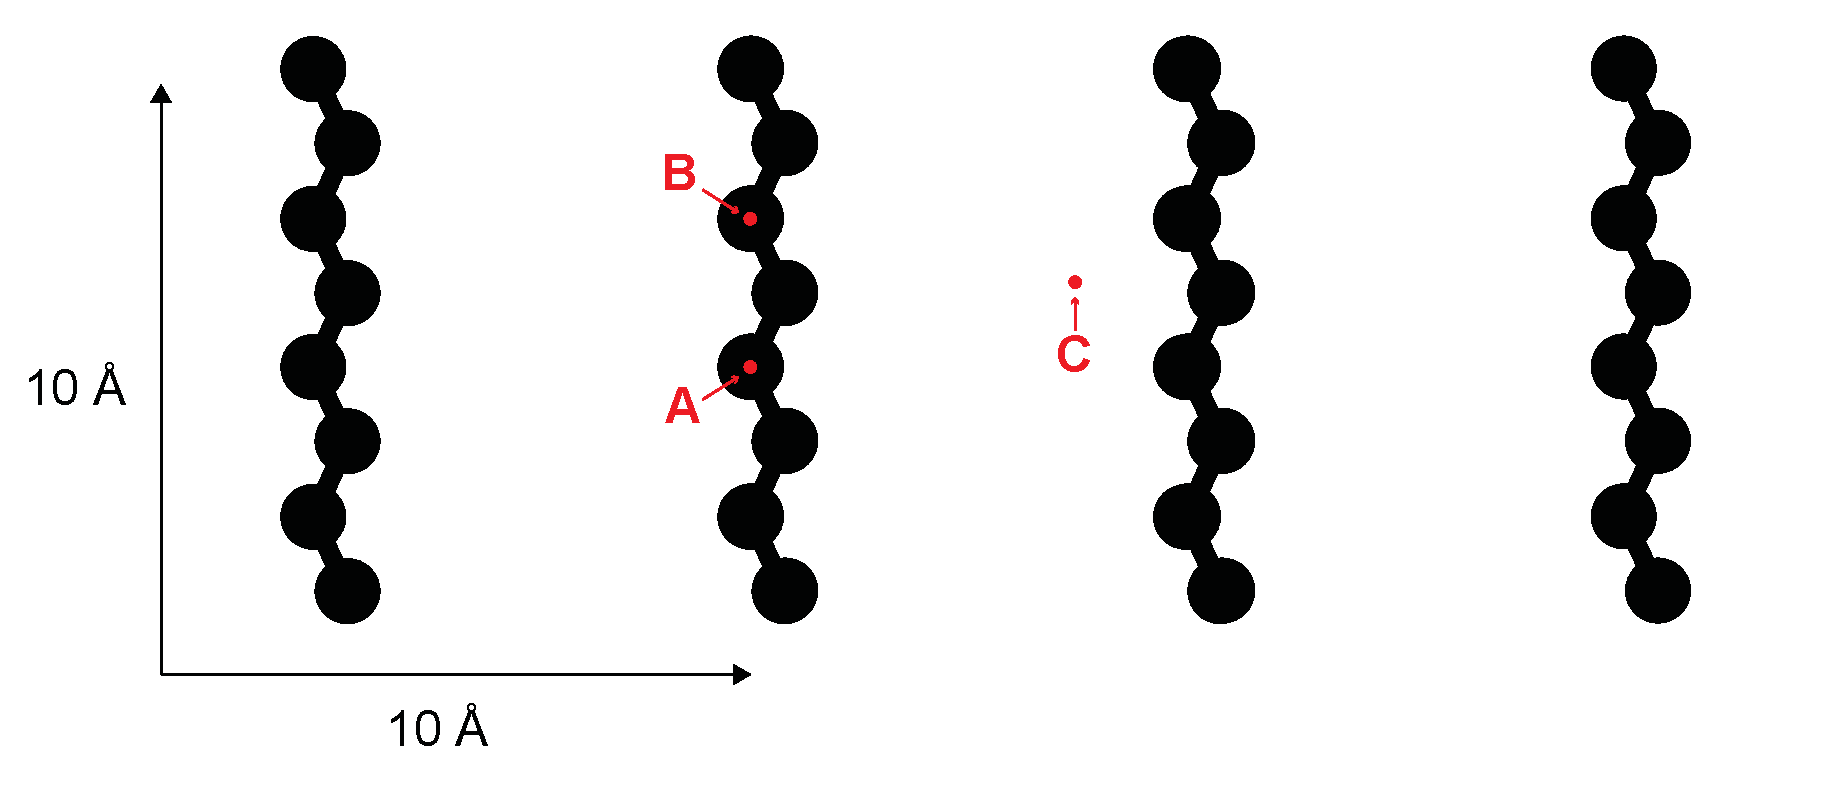
\includegraphics[width=0.6\textwidth]{\figpath/Model1_PE_layer.pdf}}	
	
	For simplicity, only the carbon atoms are shown.
	
\end{model}


\begin{ctqs}

%	\question Explain, in your own words, how the chains of polyethylene are arranged in the crystal.
%	
%		\begin{solution}[1.5in]
%		\end{solution}

	\question Imagine you are able to shrink yourself down to the atomic scale and walk around on the layer of poly(ethylene) chains shown in the second half of the model.
	
		\begin{enumerate}
			\item If you start at point A and walk to point B, will it look like your environment has changed?  Why or why not?
	
		\begin{solution}[0.75in]
		\end{solution}
			
			\item If you start at point A and walk to point C, will it look like your environment has changed?  Why or why not?
	
		\begin{solution}[0.75in]
		\end{solution}
			
		\end{enumerate}
		
	\question If you start at point A, what is the minimum distance you would need to walk \textit{in the x direction} to find an environment that looks identical to the one you started in?
	
		\begin{solution}[0.25in]
		\end{solution}
	
	\question If you start at point A, what is the minimum distance you would need to walk \textit{in the y direction} to find an environment that looks identical to the one you started in?
	
		\begin{solution}[0.25in]
		\end{solution}
	
	\question On the following image, draw lines indicating each of the minimum distance paths you identified in the previous 2 questions:

	\vspace{6pt}
	\centerline{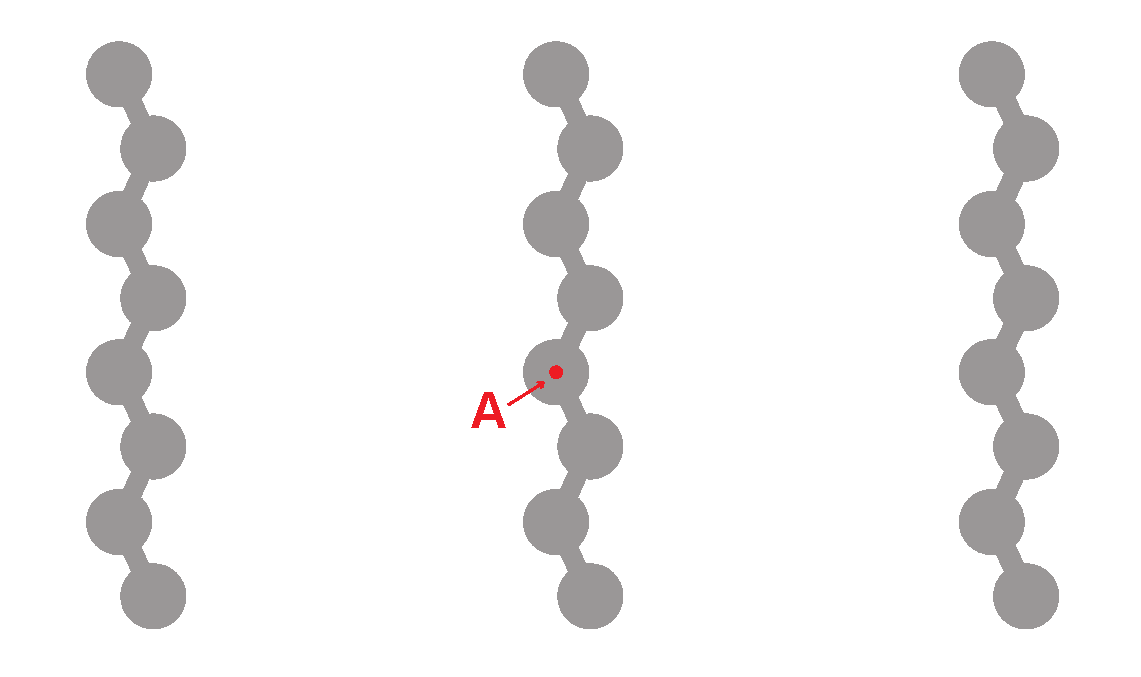
\includegraphics[width=0.35\textwidth]{\figpath/Model1_PE_layer_unitcell_blank.pdf}}	
	
	\question The two paths you drew in the previous question form two sides of a rectangle.  Why can this rectangle be thought of as the \emph{smallest repeating unit} describing a layer of a poly(ethylene) crystal?  Explain your group's reasoning in 2-3 complete sentences.
	
	\emph{(Note: feel free to draw in the other two sides of the rectangle if you find it helpful!)}
	
		\begin{solution}[1.75in]
		\end{solution}
	
\end{ctqs}

\begin{infobox}

	The smallest repeating unit of a crystal is its \emph{unit cell}.  The full, three-dimensional unit cell for the most favorable crystal structure of polyethylene is shown below:
	
	\vspace{6pt}
	\centerline{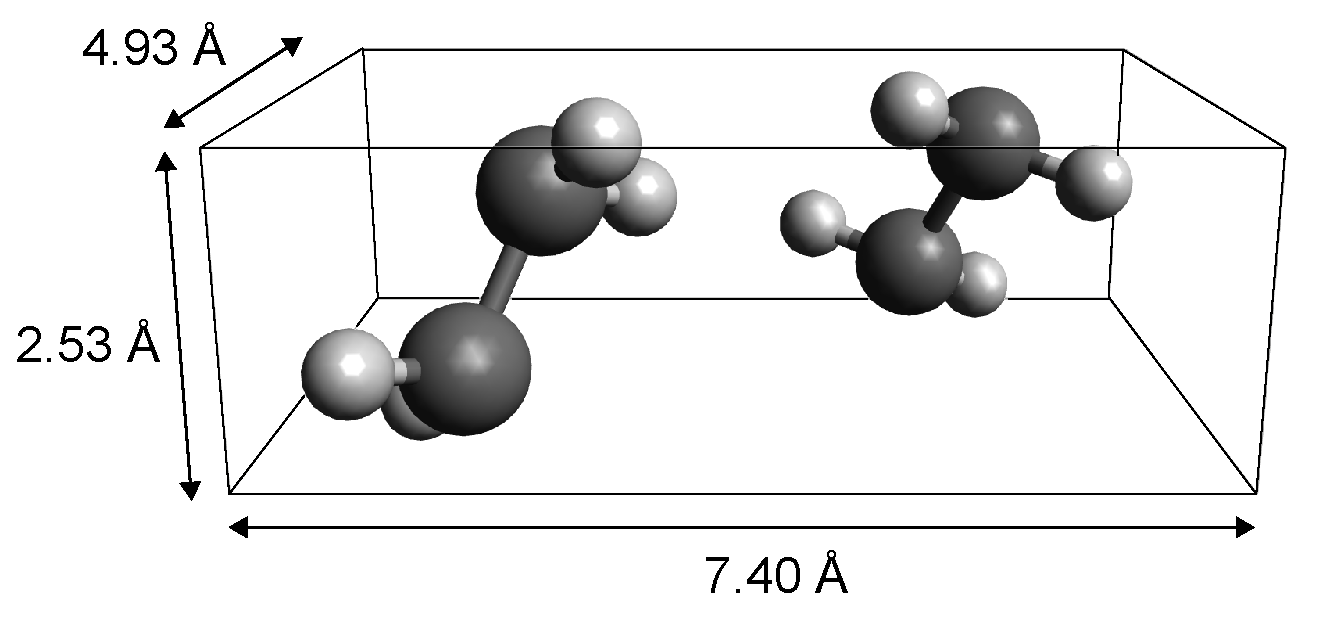
\includegraphics[width=0.4\textwidth]{\figpath/Model1_PE_unitcell_3D.pdf}}

\end{infobox}

\begin{ctqs}
	
	\question Suppose we were to add a single phenyl sidechain to the poly(ethylene) chains, as shown below.

	\vspace{6pt}
	\centerline{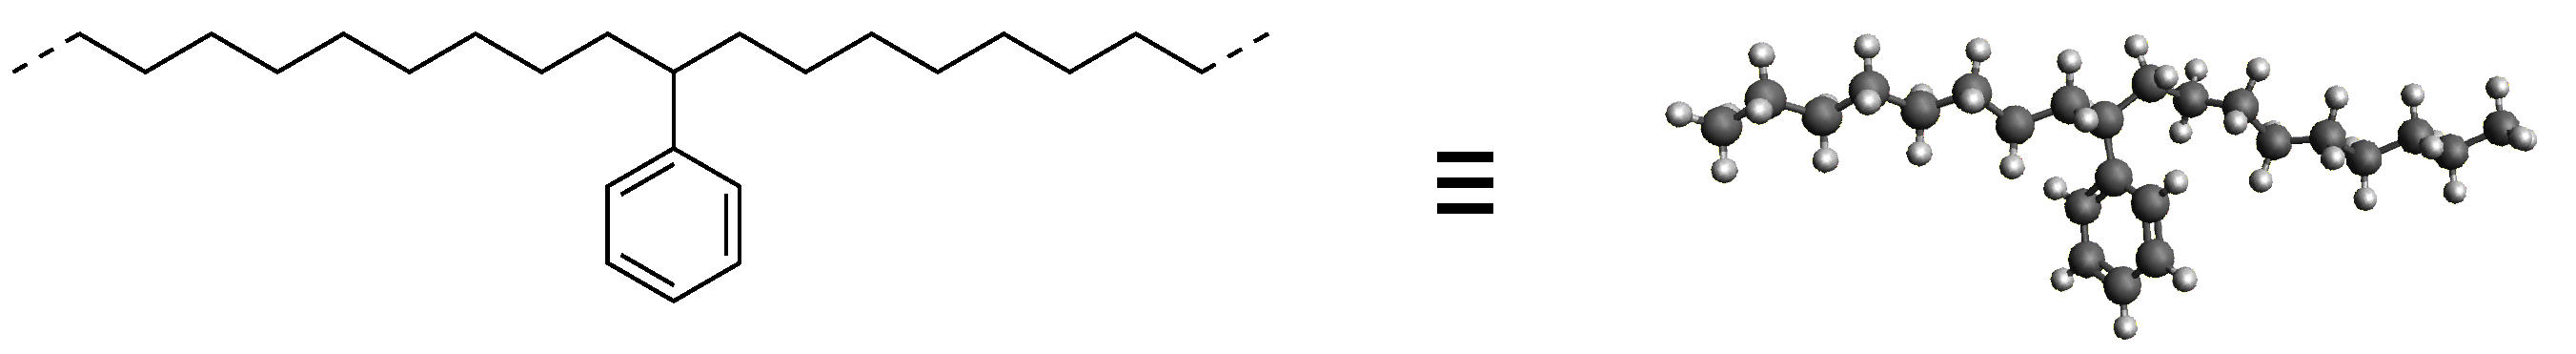
\includegraphics[width=0.8\textwidth]{\figpath/Model1_sidechain.pdf}}	
	
		\begin{enumerate}
		
			\item Would this sidechain be able to ``fit'' easily into the empty spaces in the crystal structure of polyethylene?  Briefly explain why or why not.
	
		\begin{solution}[0.5in]
		\end{solution}
			
			\item In the context of your answer to the previous question, do you expect bulky sidechains to make it easier or harder for polymer chains to crystallize?  Explain your group's reasoning in 1-2 complete sentences.
	
		\begin{solution}[1.25in]
		\end{solution}
			
		\end{enumerate}
	
	\question Briefly explain how you expect each of the following features of a polymer chain to affect its ability to pack into well-ordered crystal structures:
	
		\begin{enumerate}
		
			\item Stereoregularity (e.g. whether the polymer is isotactic, syndiotactic, or atactic)
	
		\begin{solution}[0.75in]
		\end{solution}
			
			\item Regioregularity and/or sequence regularity (e.g. how regularly sidechains and functional groups are distributed along the chains)
	
		\begin{solution}[0.75in]
		\end{solution}
			
			\item Presence of strongly polar, small sidechains that like to associate with each other
	
		\begin{solution}[0.75in]
		\end{solution}
			
		\end{enumerate}
	
\end{ctqs}

\begin{model}[Thermodynamics of Polymer Crystals]
\label{\labelbase:mdl:thermodynamics}
	
	In crystalline polymers, the crystals often form layered structures called \emph{lamellae}, which in turn organize into larger structures such as spherulites, as shown below:
	
	\vspace{6pt}
	\centerline{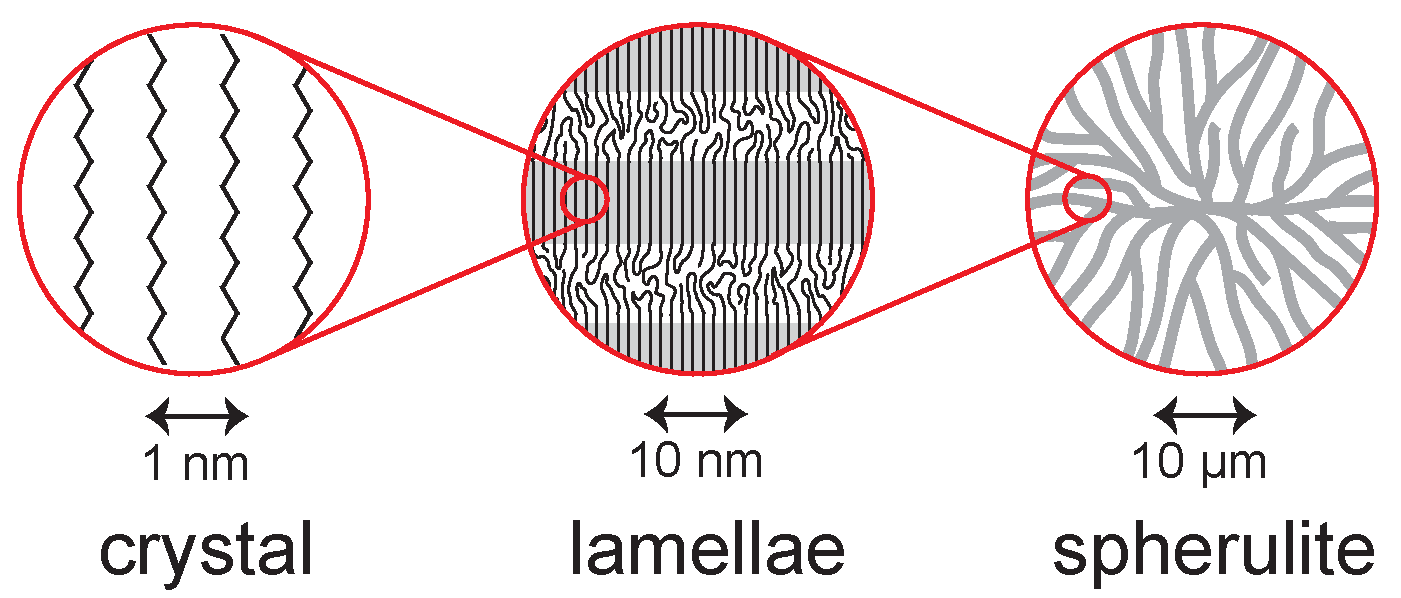
\includegraphics[width=0.8\textwidth]{\figpath/Model2_lengthscales.pdf}}
	
\end{model}

\begin{ctqs}

	\question As shown in the model, does \emph{all} of the polymer in sample form well-ordered crystals?  If not, where are more amorphous/disordered regions found?
	
		\begin{solution}[1in]
		\end{solution}
	
	\question Consider a crystal with thickness $l$ and cross-sectional area $A$ as a model for a crystalline lamella.
	
		\begin{enumerate}
		
			\item What is the volume of this crystal?
			
				\begin{solution}[0.5in]
					$V = lA$
				\end{solution}
			
			\item  If the crystal has an enthalpy per unit volume of $H^{crystal}_V$ and an entropy per unit volume of $ S^{crystal}_V$, what is the total Gibbs free energy of the crystal?
			
				\begin{solution}[0.5in]
					$G^{crystal} = lA(  H^{crystal}_V - T S^{crystal}_V )$
				\end{solution}
			
			\item If, after melting, the polymer has an enthalpy per unit volume of $H^{melt}_V$ and an entropy per unit volume of $ S^{melt}_V$, what is the total Gibbs free energy of the sample after melting?
			
				\begin{solution}[0.5in]
					$G^{melt} = lA(  H^{melt}_V - T S^{melt}_V )$
				\end{solution}
			
			\item What is the change in the Gibbs free energy of the material as the crystal melts (i.e. what is the Gibbs free energy of fusion, $\Delta G_f$)?
			
				\begin{solution}[1.25in]
					\begin{align*}
						\Delta G_f &= G^{melt} - G^{crystal} \\
							&= lA(  H^{melt}_V - T S^{melt}_V ) - lA(  H^{crystal}_V - T S^{crystal}_V ) \\
							&= lA( (H^{melt}_V - H^{crystal}_V) - T(S^{melt}_V - S^{crystal}_V) )
					\end{align*}
				\end{solution}
			
			\item The melting transition occurs at the temperature at which $\Delta G_f = 0$.  Find an expression for the melting temperature of the crystal.
			
				\begin{solution}[1.25in]
					\begin{equation*}
						T_m = \frac{H^{melt}_V - H^{crystal}_V}{S^{melt}_V - S^{crystal}_V }
					\end{equation*}
				\end{solution}
			
		\end{enumerate}


	\question The free energy of fusion depends not only on the entropy and enthalpy of the \textit{bulk} crystal, but also on the energy of surface that is in contact with the surrounding molten or amorphous polymer.
		
		If the enthalpy of the crystal surface per unit area is $H^{surf}_A = -\gamma$, what are...
	
		\begin{enumerate}
		
			\item ... the total enthalpy of the crystal before melting, including \emph{both} the bulk \emph{and} the surface contributions?
	
		\emph{Hint: remember that the crystal has \emph{two} surfaces, each with area $A$!}
		
		\begin{solution}[0.5in]
			$H = lAH_V^{crystal} - 2\gamma A$
		\end{solution}
		
			\item ... the total Gibbs free energy of the crystal before melting?
			
				\begin{solution}[0.5in]
					$G^{crystal} = lA(  H^{crystal}_V - \frac{2 \gamma}{l} - T S^{crystal}_V )$
				\end{solution}
			
			\item ... the change in Gibbs free energy upon melting?
			
				\begin{solution}[1.5in]
					\begin{align*}
						\Delta G_f %&= G^{melt} - G^{crystal} \\
							&= lA( (H^{melt}_V - \frac{2 \gamma}{l} - H^{crystal}_V) - T(S^{melt}_V - S^{crystal}_V) )
					\end{align*}
				\end{solution}
			
			\item ... and the equilibrium melting temperature?
			
				\begin{solution}[1.25in]
					\begin{equation*}
						T_m = \frac{H^{melt}_V - \frac{2 \gamma}{l} - H^{crystal}_V}{S^{melt}_V - S^{crystal}_V }
					\end{equation*}
				\end{solution}
		
		\end{enumerate} 
		
\end{ctqs}
		
\begin{infobox}
	The answer to the previous question can (if it was done correctly!) be rewritten as
		\begin{equation*}
			T_m = \frac{\Delta H^\infty_V}{\Delta S^\infty_V}\left(1-\frac{2\gamma}{l \Delta H^\infty_V}\right)
		\end{equation*}
		where
		\begin{align*}
			\Delta H^\infty_V = H^{melt}_V - H^{crystal}_V && \text{and} && \Delta S^\infty_V = S^{melt}_V - S^{crystal}_V
		\end{align*}
		
\end{infobox}
	
\begin{ctqs}	
	
	\question If $l\to\infty$, what is the melting temperature $T_m^\infty$ in terms of $\Delta H_f^\infty$, $\Delta S_f^\infty$, and any other relevant constants?
	
		\begin{solution}[0.5in]
		\end{solution}
			
	\question According to this equation, do finite-thickness lamellae usually have a higher or lower melting temperature than infinite polymer crystals?
	
		\begin{solution}[0.5in]
		\end{solution}
	
	\question Explain, in 2-3 complete sentences, how you could determine $T_m^\infty$ from data about the melting temperature of a polymer as a function of lamellar thickness.
	
		\begin{solution}[1.5in]
		\end{solution}
 
\end{ctqs}

%\begin{model}[Crystallization Kinetics]
%	\label{\labelbase:mdl:kinetics}
%
%	Most crystals form by nucleation-and-growth processes, as illustrated below:
%	
%\end{model}
%
%\begin{ctqs}
%	
%	\question \dots
%	
%\end{ctqs}

\begin{exercises}

%	\exercise Give a ``predict which of these pairs of polymers will produce the most crystalline structures'' question

	\exercise Based on the unit cell structure shown in Model \ref{\labelbase:mdl:crystalstructs}, what is the density of crystalline poly(ethylene)?
	
	\exercise In Model \ref{\labelbase:mdl:thermodynamics}, you learned how changes in the lamellar thickness impact the melting temperature of polymer crystals. A similar analysis can be used to determine how changes in polymer molecular weight impact melting temperature.  In particular, one finds that
		\begin{equation*}
			\Delta H_f\left(\frac{1}{T_m} - \frac{1}{T_m^\infty}\right) = \frac{2 R M_0}{M_n}
		\end{equation*}
		
		According to this equation, does increasing the molecular weight of a polymer generally increase or decrease its melting temperature?  Explain your reasoning in 1-2 complete sentences.
	
\end{exercises}


%\begin{problems}
%
%	\problem First exercise
%	\problem Second exercise
%	
%\end{problems}


	
\end{activity}